%\documentclass{article} % For LaTeX2e
%\usepackage{nips15submit_e,times}
%\usepackage{hyperref}
%\usepackage{url}
%\usepackage{amsmath}
%\usepackage{amssymb}
%\usepackage{amsthm}
%\usepackage{algpseudocode}
%\usepackage{algorithm}
%\usepackage{graphicx}
%\usepackage{caption}
%\usepackage{subcaption}
%\usepackage{epstopdf}
%\usepackage{float}
%%\documentstyle[nips14submit_09,times,art10]{article} % For LaTeX 2.09
%
%\newtheorem{graphconv}{Definition}
%
%
%\title{Deep Networks on Graph-Structured Data}
%
%
%\author{
%Mikael Henaff \\
%Courant Institute of Mathematical Sciences\\
%New York University\\
%\texttt{mbh305@nyu.edu} \\
%\And
%Joan Bruna \\
%University of California, Berkeley \\
%\texttt{joan.bruna@berkeley.edu} \\
%\AND
%Yann LeCun \\
%Courant Institute of Mathematical Sciences \\
%New York University \\
%\texttt{yann@cs.nyu.edu} \\
%}
%
%% The \author macro works with any number of authors. There are two commands
%% used to separate the names and addresses of multiple authors: \And and \AND.
%%
%% Using \And between authors leaves it to \LaTeX{} to determine where to break
%% the lines. Using \AND forces a linebreak at that point. So, if \LaTeX{}
%% puts 3 of 4 authors names on the first line, and the last on the second
%% line, try using \AND instead of \And before the third author name.
%
%\newcommand{\fix}{\marginpar{FIX}}
%\newcommand{\new}{\marginpar{NEW}}
%
%%\nipsfinalcopy % Uncomment for camera-ready version
%
%\begin{document}
%
%
%\maketitle
%
%\begin{abstract}
%
%\end{abstract}

\section{Experiments}
\label{experimentssect}
In order to measure the performance of spectral networks on real-world data and to explore the effect of the graph estimation procedure, we conducted experiments on three datasets from text categorization, computational biology and computer vision. All experiments were done using the Torch machine learning environment with a custom CUDA backend.

We based the spectral network architecture on that of a classical convolutional network, namely by interleaving graph convolution, ReLU and graph pooling layers, and ending with one or more fully connected layers. As noted above, training a spectral network requires an $O(N^2)$ matrix multiplication for each input and output feature map to perform the Graph Fourier Transform, compared to the efficient $O(N \text{log} N)$ Fast Fourier Transform used in classical ConvNets. We found that training the spectral networks with large numbers of feature maps to be very time-consuming and therefore chose to experiment mostly with architectures with fewer feature maps and smaller pool sizes. We found that performing pooling at the beginning of the network was especially important to reduce the dimensionality in the graph domain and mitigate the cost of the expensive Graph Fourier Transform operation.

In this section we adopt the following notation to descibe network architectures: GC$k$ denotes a graph convolution layer with $k$ feature maps, P$k$ denotes a graph pooling layer with stride $k$ and pool size $2k$, and FC$k$ denotes a fully connected layer with $k$ hidden units. In our results we also denote the number of free parameters in the network by $P_\text{net}$ and the number of free parameters when estimating the graph by $P_\text{graph}$.

\subsection{Reuters}

We used the Reuters dataset described in ~\cite{JMLR:v15:srivastava14a}, which consists of training and test sets each containing 201,369 documents from 50 mutually exclusive classes. Each document is represented as a log-normalized bag of words for 2000 common non-stop words. As a baseline we used the fully-connected network of ~\cite{JMLR:v15:srivastava14a} with two hidden layers consisting of 2000 and 1000 hidden units regularized with dropout.  

 We chose hyperparameters by performing initial experiments on a validation set consisting of one-tenth of the training data. Specifically, we set the number of subsampled weights to $k=60$, learning rate to 0.01 and used max pooling rather than average pooling. We also found that using AdaGrad ~\cite{adagrad} made training faster. All architectures were then trained using the same hyperparameters.
Since the experiments were computationally expensive, we did not train all models until full convergence. This enabled us to explore more model architectures and obtain a clearer understanding of the effects of graph construction.  

\begin{table}[H]
\caption{Results for Reuters dataset. Accuracy is shown at epochs 200 and 1500.}
\begin{center}
\begin{tabular}{|c|c|c|c|c|c|}
\hline
Graph & Architecture & $P_\text{net}$ & $P_\text{graph}$ & Acc. (200) & Acc. (1500)\\
\hline
- &FC2000-FC1000 & $6 \cdot 10^6$ & 0 &70.18 \footnotemark & 70.18 \\
Supervised & GC4-P4-FC1000 & $2\cdot 10^6$ & $2 \cdot 10^6$ & 69.41 & 70.03 \\
Supervised & GC8-P8-FC1000 & $2 \cdot 10^6$ & $2 \cdot 10^6$ & 69.15 & - \\
Supervised low rank & GC4-P4-FC1000 & $2\cdot 10^6$ & $5 \cdot 10^5$ & 69.25 & - \\
Supervised low rank & GC8-P8-FC1000 & $2 \cdot 10^6$ & $5 \cdot 10^5$ & 68.35 & - \\
Supervised & GC16-P4-GC16-P4-FC1000& $2 \cdot 10^6$ & $2 \cdot 10^6$ & 69.04 & - \\
Supervised &GC64-P8-GC64-P8-FC1000 & $2 \cdot 10^6$ & $2 \cdot 10^6$ & 69.09 & - \\
RBF kernel & GC4-P4-FC1000 & $2\cdot 10^6$ & $2 \cdot 10^6$ & 67.85 & - \\
RBF kernel & GC8-P8-FC1000 & $2 \cdot 10^6$ & $2 \cdot 10^6$ & 66.95 & - \\
RBF kernel & GC16-P4-GC16-P4-FC1000 & $2 \cdot 10^6$ & $2 \cdot 10^6$ & 67.16 & - \\
RBF kernel & GC64-P8-GC64-P8-FC1000 & $2 \cdot 10^6$ & $2 \cdot 10^6$ & 67.42 & - \\
RBF kernel (local)& GC4-P4-FC1000 & $2\cdot 10^6$ & $2 \cdot 10^6$ & 68.56 & - \\
RBF kernel (local) & GC8-P8-FC1000 & $2 \cdot 10^6$ & $2 \cdot 10^6$ & 67.66 & - \\
\hline
\end{tabular}
\end{center}
\label{reuterstable}
\end{table}
\footnotetext{this is the maximum value before the fully connected starts overfitting}
%\begin{figure}[h]
%\begin{center}
%\includegraphics[width=0.4\textwidth]{{reuters_fc_vs_spectral}.pdf}
%\caption{Results on Reuters.}
%\end{center}
%\end{figure}
%\label{merckfigure}

Note that our architectures are designed so that they factor the first hidden layer of the fully connected network across feature maps and a subsampled graph, trading off resolution in the graph domain for resolution across feature maps. The number of inputs into the last fully connected layer is always the same as for the fully-connected network. The idea is to reduce the number of parameters in the first layer of the network while avoiding too much compression in the second layer. 
We note that as we increase the tradeoff between resolution in the graph domain and across features, there reaches a point where performance begins to suffer. This is especially pronounced for the unsupervised graph estimation strategies. When using the supervised method, the network is much more robust to the factorization of the first layer. Table \ref{reuterstable} compares the test accuracy of the fully connected network and the GC4-P4-FC1000 network. Figure \ref{merckfigure}-left shows that the factorization of the lower layer has a beneficial regularizing effect. 

\begin{figure}
       \centering
        \includegraphics[width=0.25\textwidth]{{reuters_alpha_0.01_global}.pdf}
         \includegraphics[width=0.25\textwidth]{{reuters_alpha_0.01_local}.pdf} \\
          \includegraphics[width=0.25\textwidth]{{merck3_alpha_0.01_global}.pdf}
          \includegraphics[width=0.25\textwidth]{{merck3_alpha_0.01_local}.pdf}
       \caption{Similarity graphs for the Reuters (top) and Merck DPP4 (bottom) datasets. Left plots correspond to global $\sigma$, right plots to local $\sigma$.}\label{fig:animals}
\end{figure}


%\begin{figure}
%       \centering
%       \begin{subfigure}[b]{0.3\textwidth}
%               \includegraphics[width=1\textwidth]{{reuters_alpha_0.01_global}.pdf}
%               \caption{Global scaling..}
%       \end{subfigure}%
%       ~ %add desired spacing between images, e. g. ~, \quad, \qquad, \hfill etc.
%         %(or a blank line to force the subfigure onto a new line)
%       \begin{subfigure}[b]{0.3\textwidth}
%               \includegraphics[width=1\textwidth]{{reuters_alpha_0.01_local}.pdf}
%               \caption{Local scaling.}
%       \end{subfigure}
%       
%       \begin{subfigure}[b]{0.3\textwidth}
%               \includegraphics[width=1\textwidth]{{merck3_alpha_0.01_global}.pdf}
%               \caption{Global scaling.}
%       \end{subfigure}%
%       ~ %add desired spacing between images, e. g. ~, \quad, \qquad, \hfill etc.
%         %(or a blank line to force the subfigure onto a new line)
%       \begin{subfigure}[b]{0.3\textwidth}
%               \includegraphics[width=1\textwidth]{{merck3_alpha_0.01_local}.pdf}
%               \caption{Local scaling.}
%       \end{subfigure}
%       \caption{Similarity graphs for the Reuters (top) and Merck DPP4 (bottom) datasets.}\label{fig:animals}
%\end{figure}


\subsection{Merck Molecular Activity Challenge}

The Merck Molecular Activity Challenge is a computational biology benchmark where the task is to predict activity levels for various molecules based on the distances in bonds between different atoms. For our experiments we used the DPP4 dataset which has 8193 samples and 2796 features. We chose this dataset because it was one of the more challenging and was of relatively low dimensionality which made the spectral networks tractable. As a baseline architecture, we used the network of ~\cite{Ma:JournalChem2015} which has 4 hidden layers and is regularized using dropout and weight decay. We used the same hyperparameter settings and data normalization recommended in the paper.   

As before, we used one-tenth of the training set to tune hyperparameters of the network. For this task we found that $k=40$ subsampled weights worked best, and that average pooling performed better than max pooling. Since the task is to predict a continuous variable, all networks were trained by minimizing the Root Mean-Squared Error loss. Following ~\cite{Ma:JournalChem2015}, we measured performance by computing the squared correlation between predictions and targets.

\begin{figure}[h]
\begin{center}
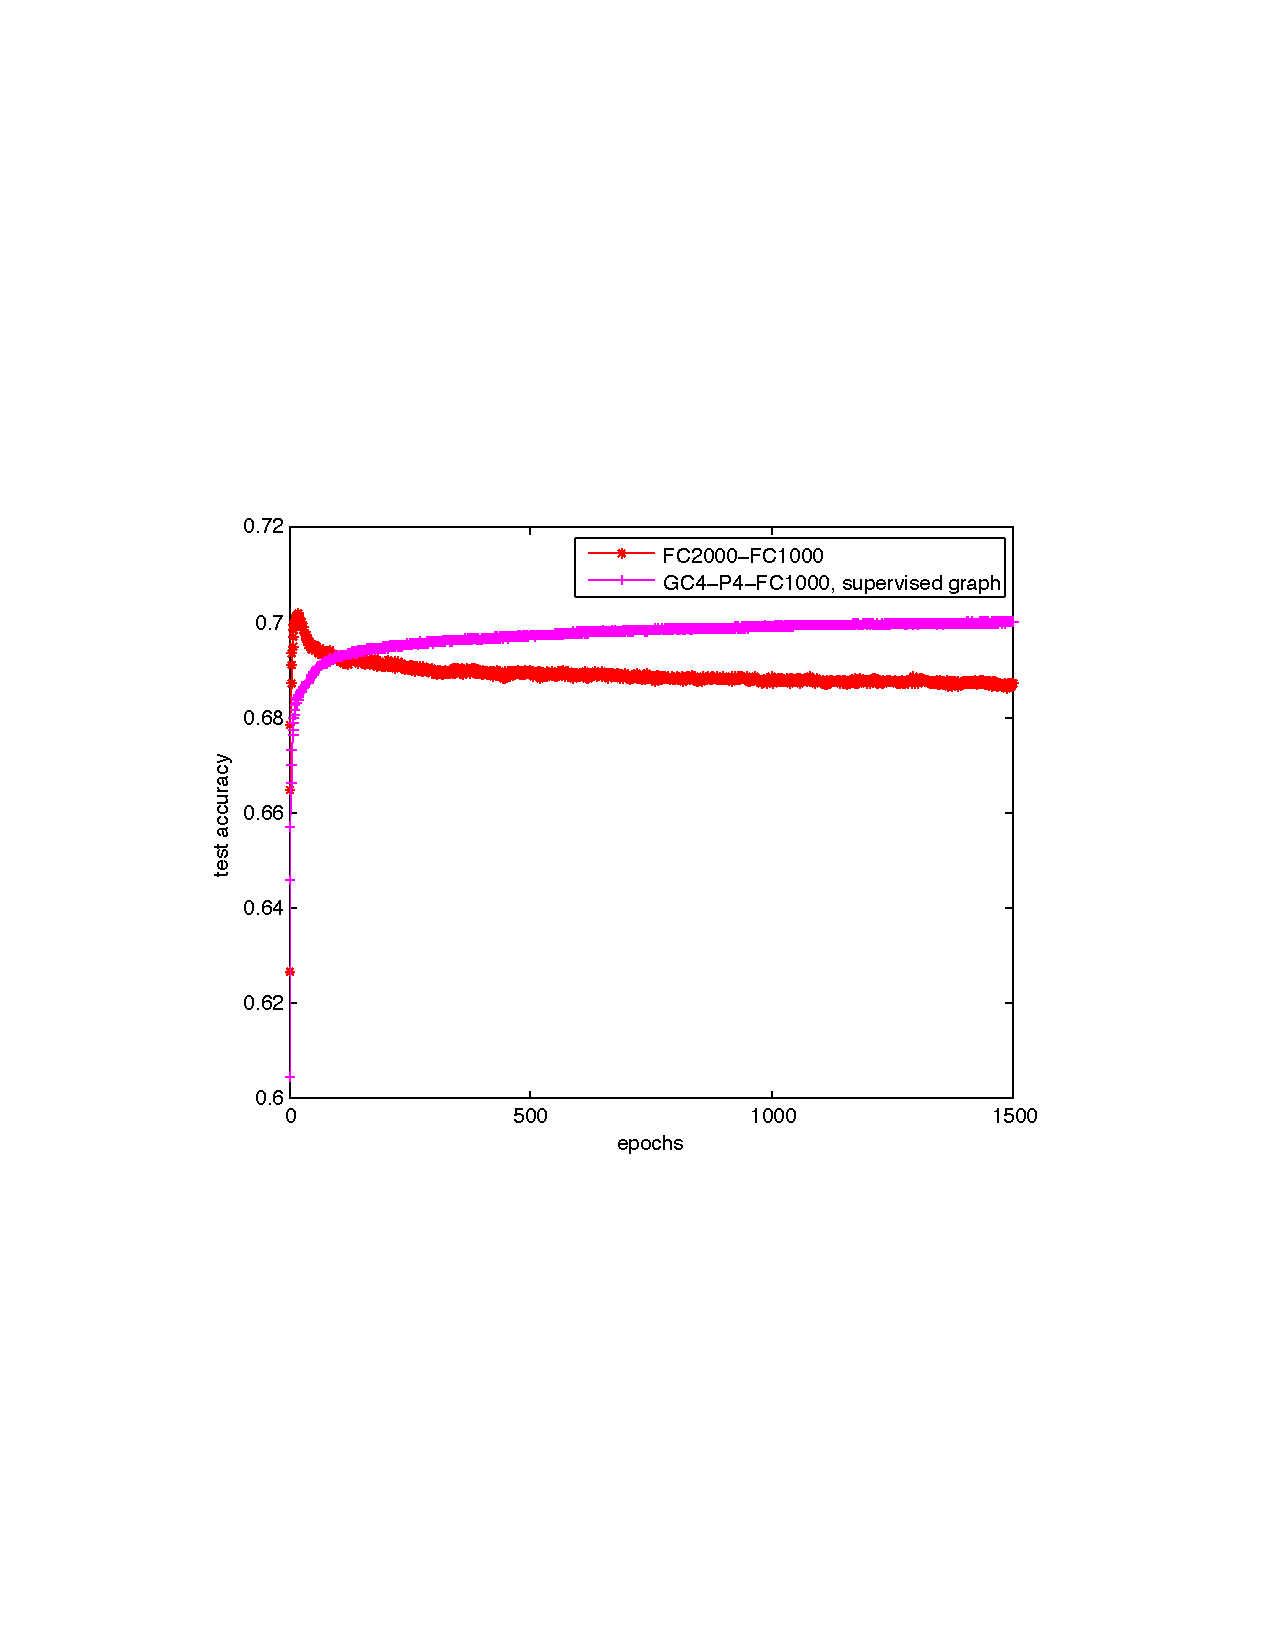
\includegraphics[width=0.4\textwidth]{reuterscrop.pdf}~
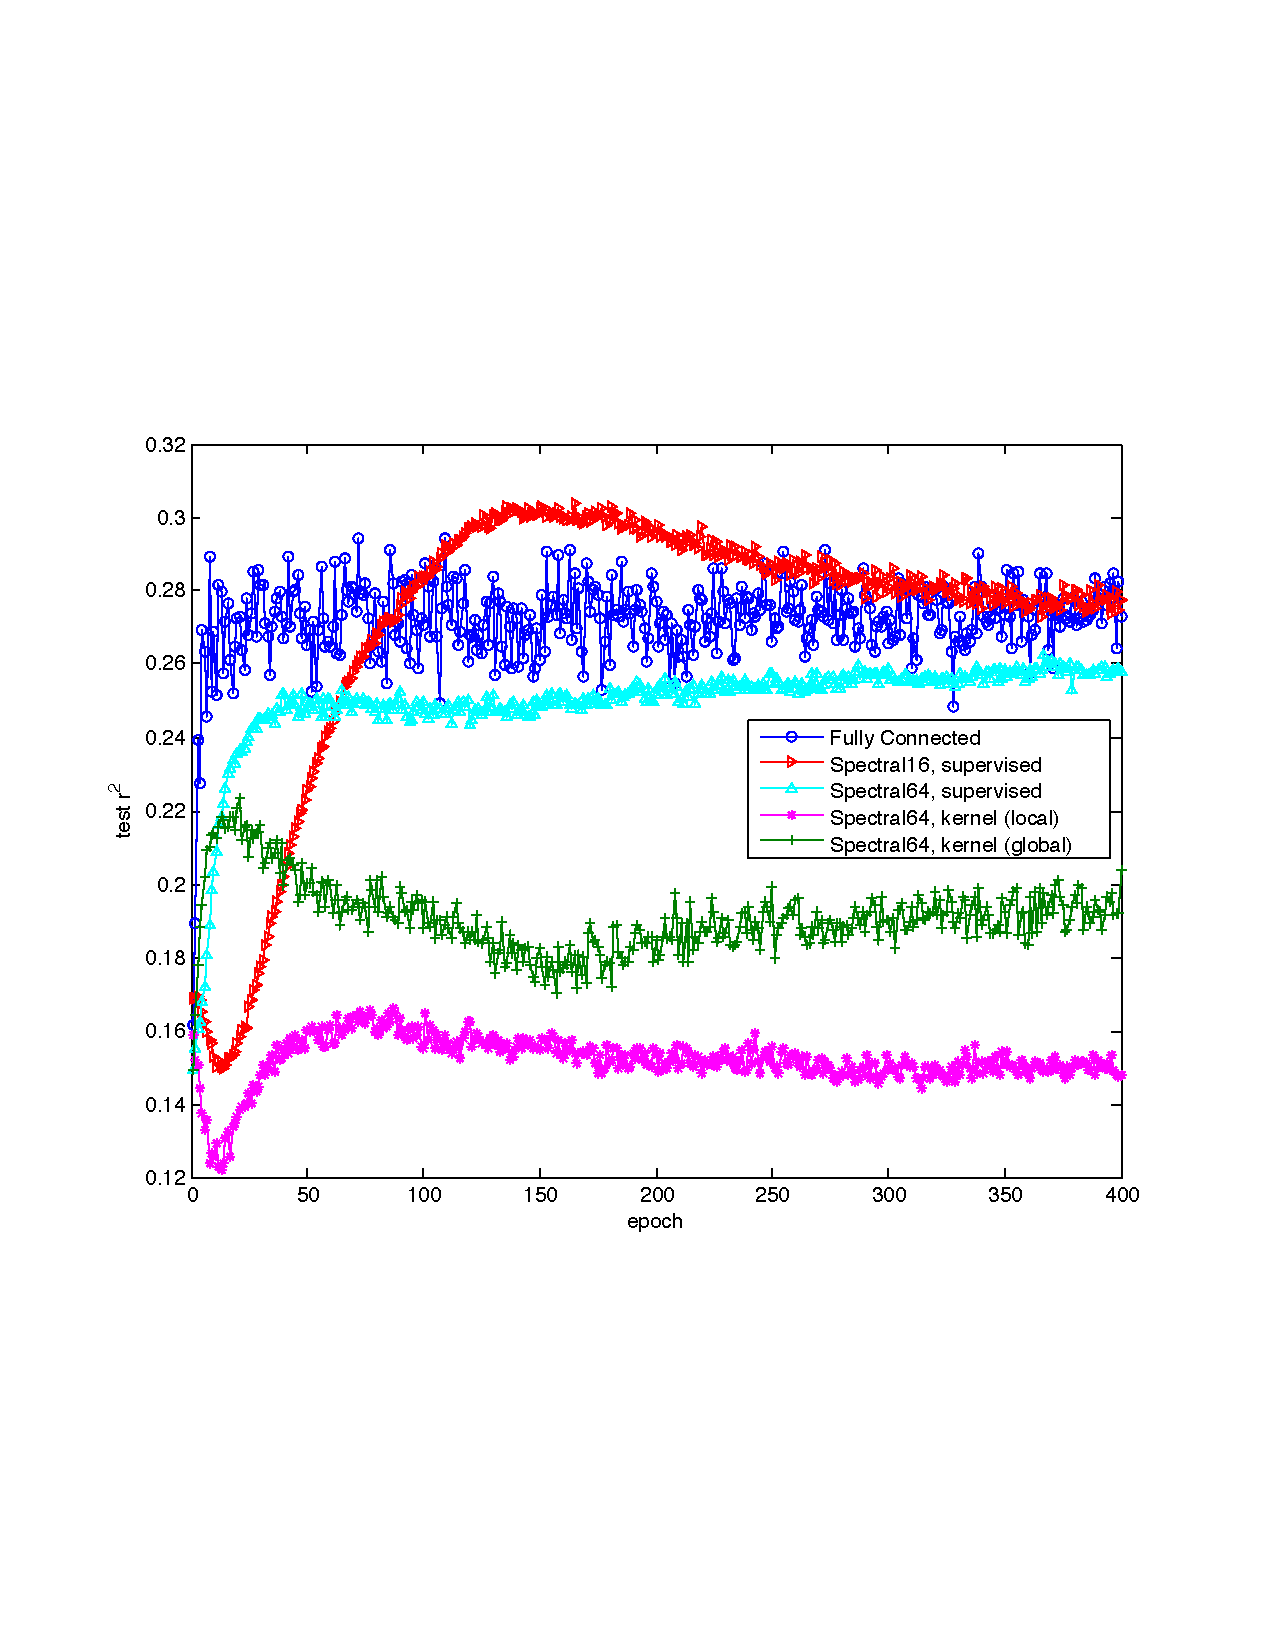
\includegraphics[width=0.4\textwidth]{merckcrop.pdf}
\caption{Evolution of Test accuracy. Left: Reuters dataset, Right: Merck dataset.}
\end{center}
\end{figure}
\label{merckfigure}


\begin{table}[H]
\caption{Results for Merck DPP4 dataset.}
\begin{center}
\begin{tabular}{|c|c|c|c|c|}
\hline
Graph & Architecture & $P_\text{net}$ & $P_\text{graph}$ & $R^2$\\ 
\hline
- &FC4000-FC2000-FC1000-FC1000 & $22.1 \cdot 10^6$ & 0 & 0.2729 \\
Supervised & GC16-P4-GC16-P4-FC1000-FC1000 & $3.8\cdot 10^6$ & $3.9 \cdot 10^6$ & 0.2773 \\
Supervised & GC64-P8-GC64-P8-FC1000-FC1000 & $3.8\cdot 10^6$ & $3.9 \cdot 10^6$ &0.2580 \\
RBF Kernel & GC64-P8-GC64-P8-FC1000-FC1000 & $3.8\cdot 10^6$ & $3.9 \cdot 10^6$ &0.2037 \\
RBF Kernel (local) & GC64-P8-GC64-P8-FC1000-FC1000 & $3.8\cdot 10^6$ & $3.9 \cdot 10^6$  &0.1479 \\
\hline
\end{tabular}
\end{center}
\end{table}

We again designed our architectures to factor the first two hidden layers of the fully-connected network across feature maps and a subsampled graph, and left the second two layers unchanged. As before, we see that the unsupervised graph estimation strategies yield a significant drop in performance whereas the supervised strategy enables our network to perform similarly to the fully-connected network with much fewer parameters. This indicates that it is able to factor the lower-level representations in such a way as to retain useful information for the classification task.

Figure \ref{merckfigure}-right shows the test performance as the models are being trained. We note that the Merck datasets have test set samples assayed at a different time than the samples in the training set, and thus the distribution of features is typically different between the training and test sets. Therefore the test performance can be a significantly noisy function of the train performance. However, the effect of the different graph estimation procedures is still clear. 

\subsection{ImageNet}

In the experiments above our graph construction relied on estimation from the data. 
To measure the influence of the graph construction compared to the filter learning in the graph frequency domain, we performed the same experiments on the ImageNet dataset for which the graph is already known, namely it is the 2-D grid. The spectral network was thus a convolutional network whose weights were defined in the frequency domain using frequency smoothing rather than imposing compactly supported filters.
 Training was performed exactly as in Figure 1, except that the linear transformation was a Fast Fourier Transform. 

Our network consisted of 4 convolution/ReLU/max pooling layers with 48, 128, 256 and 256 feature maps, followed by 3 fully-connected layers each with 4096 hidden units regularized with dropout. We trained two versions of the network: one classical convolutional network and one as a spectral network where the weights were defined in the frequency domain only and were interpolated using a spline kernel. Both networks were trained for 40 epochs over the ImageNet dataset where input images were scaled down to $128 \times 128$ to accelerate training.  

\begin{table}[H]
\caption{ImageNet results}
\begin{center}
\begin{tabular}{|c|c|c|c|}
\hline
Graph & Architecture & Test Accuracy (Top 5) & Test Accuracy (Top 1)\\
\hline
2-D Grid & Convolutional Network & 71.854 & 46.24\\
2-D Grid & Spectral Network & 71.998 & 46.71\\
\hline
\end{tabular}
\end{center}
\end{table}

\begin{figure}[h]
\centering
 \includegraphics[width=0.5\textwidth]{{imagenetcrop}.pdf}
 \caption{ConvNet vs. SpectralNet on ImageNet.}
\end{figure}



We see that both models yield nearly identical performance. Interstingly, the spectral network learns faster than the ConvNet during the first part of training, although both networks converge around the same time. This requires further investigation.


%
%\bibliography{references}{}
%\bibliographystyle{plain}
%
%\end{document}
